\pdfoutput=1
\documentclass[10pt,twocolumn,aps,superscriptaddress, floatfix,notitlepage]{revtex4-1}
\usepackage{amsmath,cases}
\usepackage[utf8]{inputenc}
\DeclareUnicodeCharacter{2215}{/}
\usepackage{isotope}
\usepackage[T1]{fontenc}
\usepackage{lmodern}
\usepackage{graphicx}
\usepackage{amsmath}
\usepackage{amssymb}
\DeclareRobustCommand{\bbone}{\text{\usefont{U}{bbold}{m}{n}1}}
\DeclareMathOperator{\EX}{\mathbb{E}}% expected value
\usepackage{scalerel}
% \usepackage{wasysym}
\usepackage{bm}
\usepackage[dvipsnames]{xcolor}
\usepackage[colorlinks, citecolor={blue!50!black}, urlcolor={blue!50!black}]{hyperref}
\usepackage{bookmark}
\usepackage{tabularx}
\usepackage{mathtools}
\usepackage{microtype}
\usepackage[version=4]{mhchem}
\usepackage{bbm}
\usepackage[justification = raggedright]{caption}
\usepackage[singlelinecheck=off,justification=justified]{subcaption}


\usepackage{braket}
\usepackage{mathtools}

\usepackage[normalem]{ulem}
\usepackage{layouts}
\usepackage{float}

\graphicspath{{./}}

% A `comment' command to keep track of the narrative; uncomment it and comment the following chunk to hide the paragraphs from TOC.
\newcommand{\co}[1]{\paragraph{#1}}
% % Add to ToC
 \setcounter{secnumdepth}{5}
 \setcounter{tocdepth}{5}
% \renewcommand{\paragraph}[1]{%
%   \par\refstepcounter{paragraph}% Increase section counter
%   \paragraphmark{#1}% Add section mark (header)
%   \addcontentsline{toc}{paragraph}{\protect\numberline{\theparagraph}#1}% Add section to ToC
%   % Add more content here, if needed.
% }
\bibliographystyle{chicago}

\begin{document}

\title{Design and simulation of a Majorana trijunction}

\begin{abstract}

\end{abstract}
\maketitle

%-----------------------------------------

\section{Introduction}

\textit{a) Precise manipulation of at least three Majorana bound states is required to have a topological qubit.} Majorana bound states (MBS) appear as the zero-energy degenerated manifold of a topological superconductor where particle-hole symmetry, along with their non-local wavefunction, makes them robust against local sources of noise. MBS can be used to define a topological qubit, which requires at least three MBS with precisely controlled interactions between each pair\cite{Aasen2016}. There are two main approaches to defining and operating a topological qubit. On one hand, braiding MBS around each other along gate-defined paths can be used to perform operations in a given parity subspace\cite{Sau2011,Alicea2011,Bauer2018,Zhou2021}. On the other hand, joint parity measurements of different pairs of MBS is equivalent to braiding\cite{Plugge2017,Li2018,Hell2016,Karzig2017}. The later approach offers simpler device configuration, and, consequently, it has been extensively studied in the context of superconducting islands with large charging energy.

\textit{b) Geometrical constraints.} To have MBS one requires a quasi-one dimensional system with low electron density, strong spin-orbit interaction, proximity induced s-wave superconducting pairing, and a magnetic field that breaks time-reversal-symmetry. For simultaneous tuning of multiple nanowires to the topological phase is sensitive to angle variations that may lead to destruction of MBS. To avoid such fine tuning, we require that all nanowires must be parallel to the magnetic field.

\textit{c) Gate defined ballistic cavities.}  Three MBS come together to the cavity, and their interaction is mediated by the cavity states. Ballistic cavities have been extensively studied in the context of semi-classical physics. The conductance depends on the classical trajectories that can be drawn inside the cavity\cite{Zhang2017,Nazmitdinov2002,Wirtz1997}. This problem is similar to the trijunction design. Here, the leads are Majorana nanowires. In the cavity there is a spin-orbit interaction and TRS is broken. Such devices can be created in two-dimensional electron gases\cite{Moehle2021} where the nanowires and the cavity can be created in a single device. The control and separation of different regions is achieved by electrostatic gates\cite{Hell2017}. {\color{red} Discuss about geometry of trijunction in gate-defined and etching-defined structures. Pros and cons.}

\textit{d) } In this work we consider a trijunction of Majorana nanowires connected by a semiconducting ballistic cavity. Consider simple geometrical shapes for the cavity and multi-channel topological leads, we calculate the coupling of all pairs of MBS at the phase sweet-spot in the strong-coupling regime where there are no barriers between the leads and the cavity. We show from our simulations that the geometry allows us to choose which pair of MBS has the largest coupling. We explore if this result can be explained by looking at the properties of the cavity states. {\color{red} Specifically, we look at the trajectories defined by a local Fourier transform, and at the localisation of the wavefunctions via the inverse participation ratio (IPR)}. Finally, we propose and simulate an electrostatic gate configuration for controlling the trijunction in a two-dimensional electron gas system using a Poisson solver.

\section{Methods}

\textit{Tight-binding Hamiltonian.} Let us consider a system defined by the Hamiltonian,
\begin{multline}
\mathcal H = \left[ U(x,y) - \frac{\hbar^2}{2m_e} (\partial_x^2 + \partial_y^2)  \right] \sigma_0 \tau_z + \Delta (x,y) e^{i \phi(x, y)} \sigma_0 \tau_x \\ + E_Z  \sigma_y \tau_0 + \alpha( p_x \sigma_y - p_y \sigma_x)\tau_z,
\end{multline}
where $U(x,y)$ is the electrostatic potential, $\Delta(x,y)$ is a the s-wave superconducting gap defined only in the wires region, $\phi(x,y)$ is the superconducting phase that is constant along each wire, but varies for all of them, $\alpha$ the strength of the spin-orbit, $\mu(x,y)$ is the chemical potential that is different for each wire and for the cavity, and $E_Z$ as the Zeeman energy. This Hamiltonian is discretised over a 2D domain and solved using kwant. The phase $\phi$ has been tuned such that the coupling of each pair of MBS is maximum. {\color{red}This value is the same for all geometries. There should be a simple argument from which to derive this value.}

The coupling is calculated by diagonalising a finite system and extracting the eigenvalue that corresponds to the MBS next to the cavity. We repeat this calculation for each pair of MBS and tune the system at the optimal point for each one.

\textit{Poisson solver}

\textit{Geometries}  We consider the shapes shown in Fig. \ref{fig:shapes} to study the geometry dependence of the coupling between different pairs of MBS. We can classify them as:

\begin{figure}[!h]
  \centering
  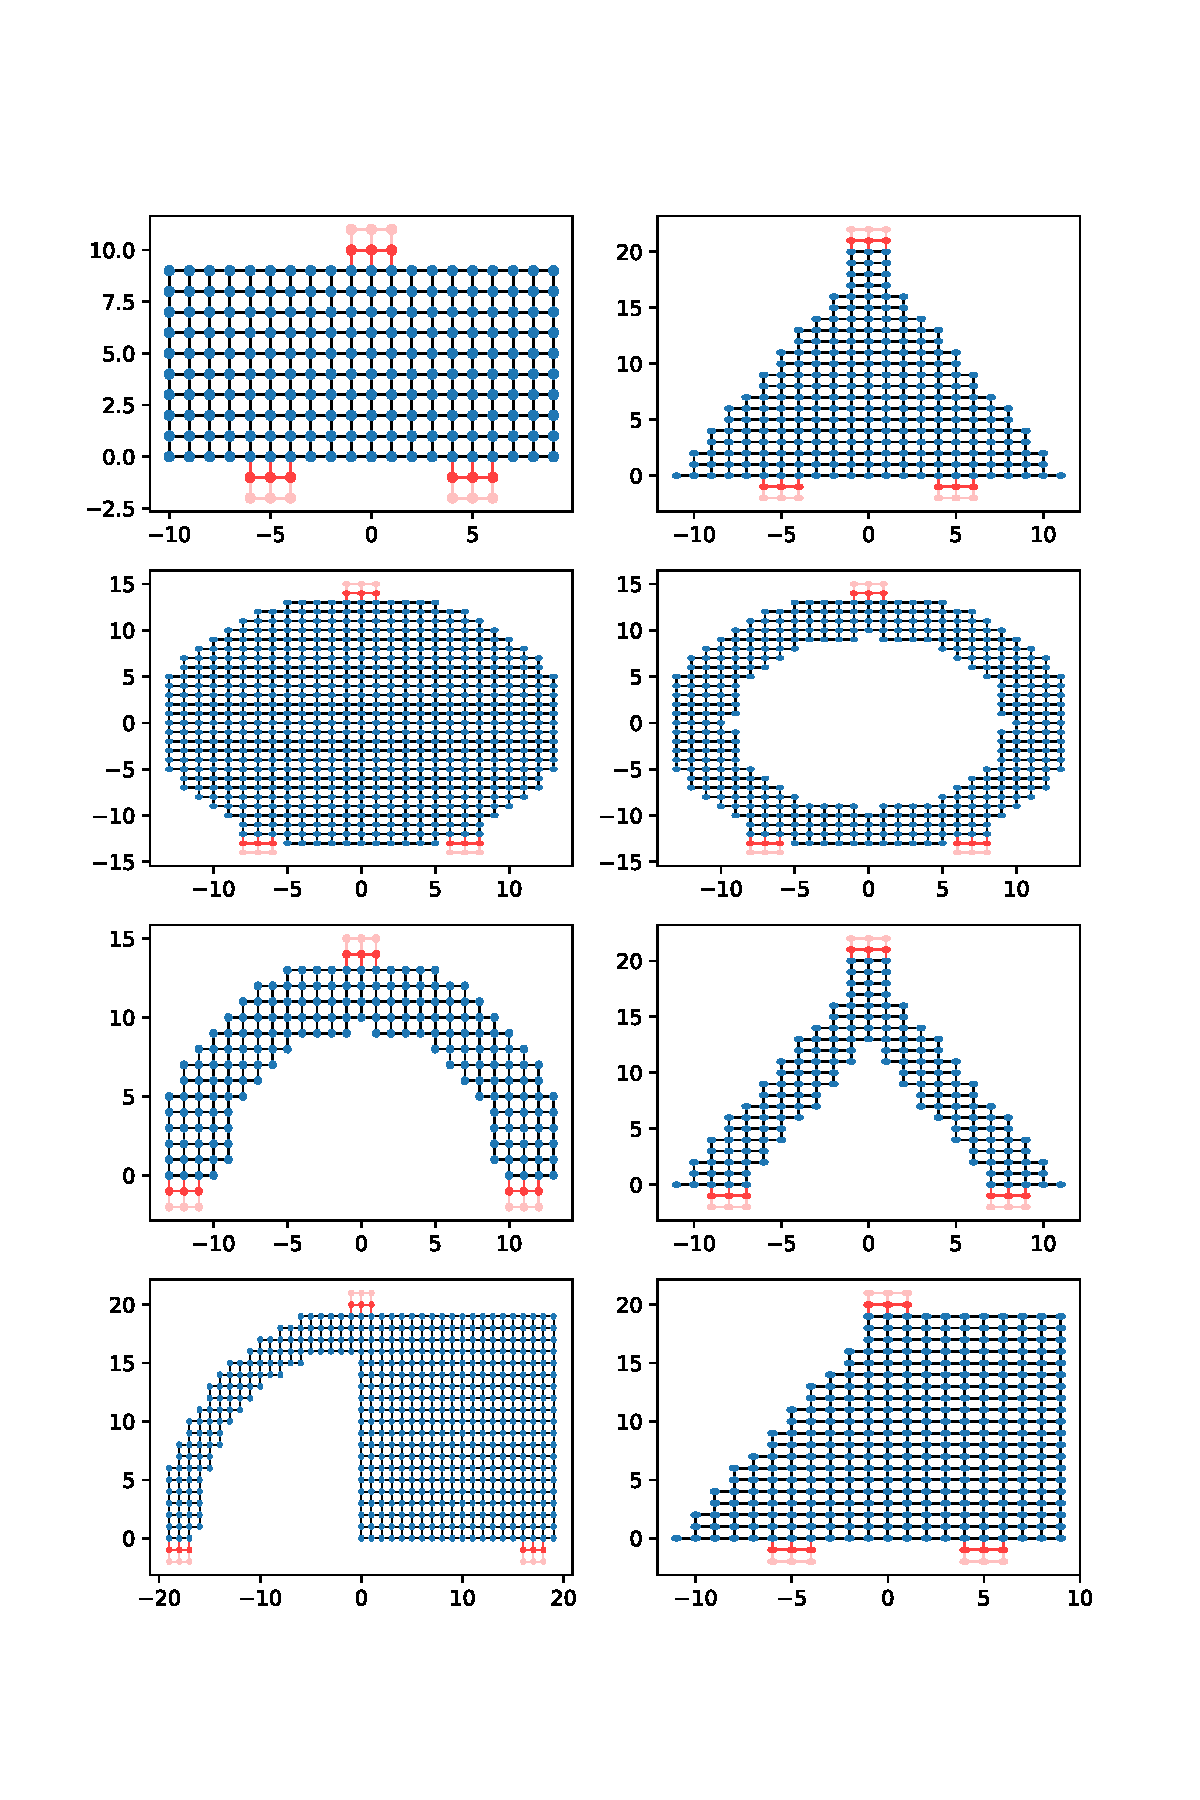
\includegraphics[width=0.9\linewidth]{figures/shapes.pdf}
  \caption{Illustrative representation of trijunction shapes.}
  \label{fig:shapes}
\end{figure}

\begin{enumerate}
\item Broad shapes with fixed structure. That is, shapes that can only be changed by increasing or decreasing its size and that have a broad scattering regions. For example, a rectangle or a circle.
\item Narrow shapes with fixed structure. Similar to the previous case, but the scattering region is narrowly defined between the boundaries. For example, a ring.
\item Broad shapes with parametric structure. That is, shapes whose structure can be controlled by a parameter. Variation of such parameter changes qualitatively the coupling behaviour. For example, a triangle with varying diagonal angle.
\item Narrow shapes with parametric structure. For example, a V-shape.
\end{enumerate}

\section{Results}

The trijunction is first modeled without an electrostatic environment. The chemical potential is a step function defined over the different regions of the system. No barriers are placed between the cavity and the leads. The phase is tuned such that the coupling is maximised. I show here results for a half ring geometry and for a triangular geometry with different angles. The labeling of the wires is: left-1, right-2, top-3. So $E_{ij}$ corresponds to the coupling energy of the $i$-th and $j$-th MBS. The nanowires have a finite width of $90$nm. We repeat the calculation for all sub bands that have MBS.

\subsection{Narrow geometries}

Let us recall that in a ballistic system, the only sources of scattering are the boundaries of the system. In a narrow system, electronic trajectories starting at a lead will scatter from the boundaries many times until reach the other lead. Therefore, narrow shapes will have small couplings between all pairs of Majoranas. That is the case show in Fig \ref{fig:half_ring} where the coupling of all MBS pairs is calculated as a function of the cavity chemical potential for a half ring geometry in the strong coupling regime. One can observe that for a small cavity, top plot, the largest coupling is $E_{23}$ and $E_{13}$, i.e. right-middle and left-middle MBS. As we increase the size of the system, the coupling between the far MBS, $E_{12}$, becomes comparable to that of the closer pairs.

\begin{figure}[h!]
  \centering
  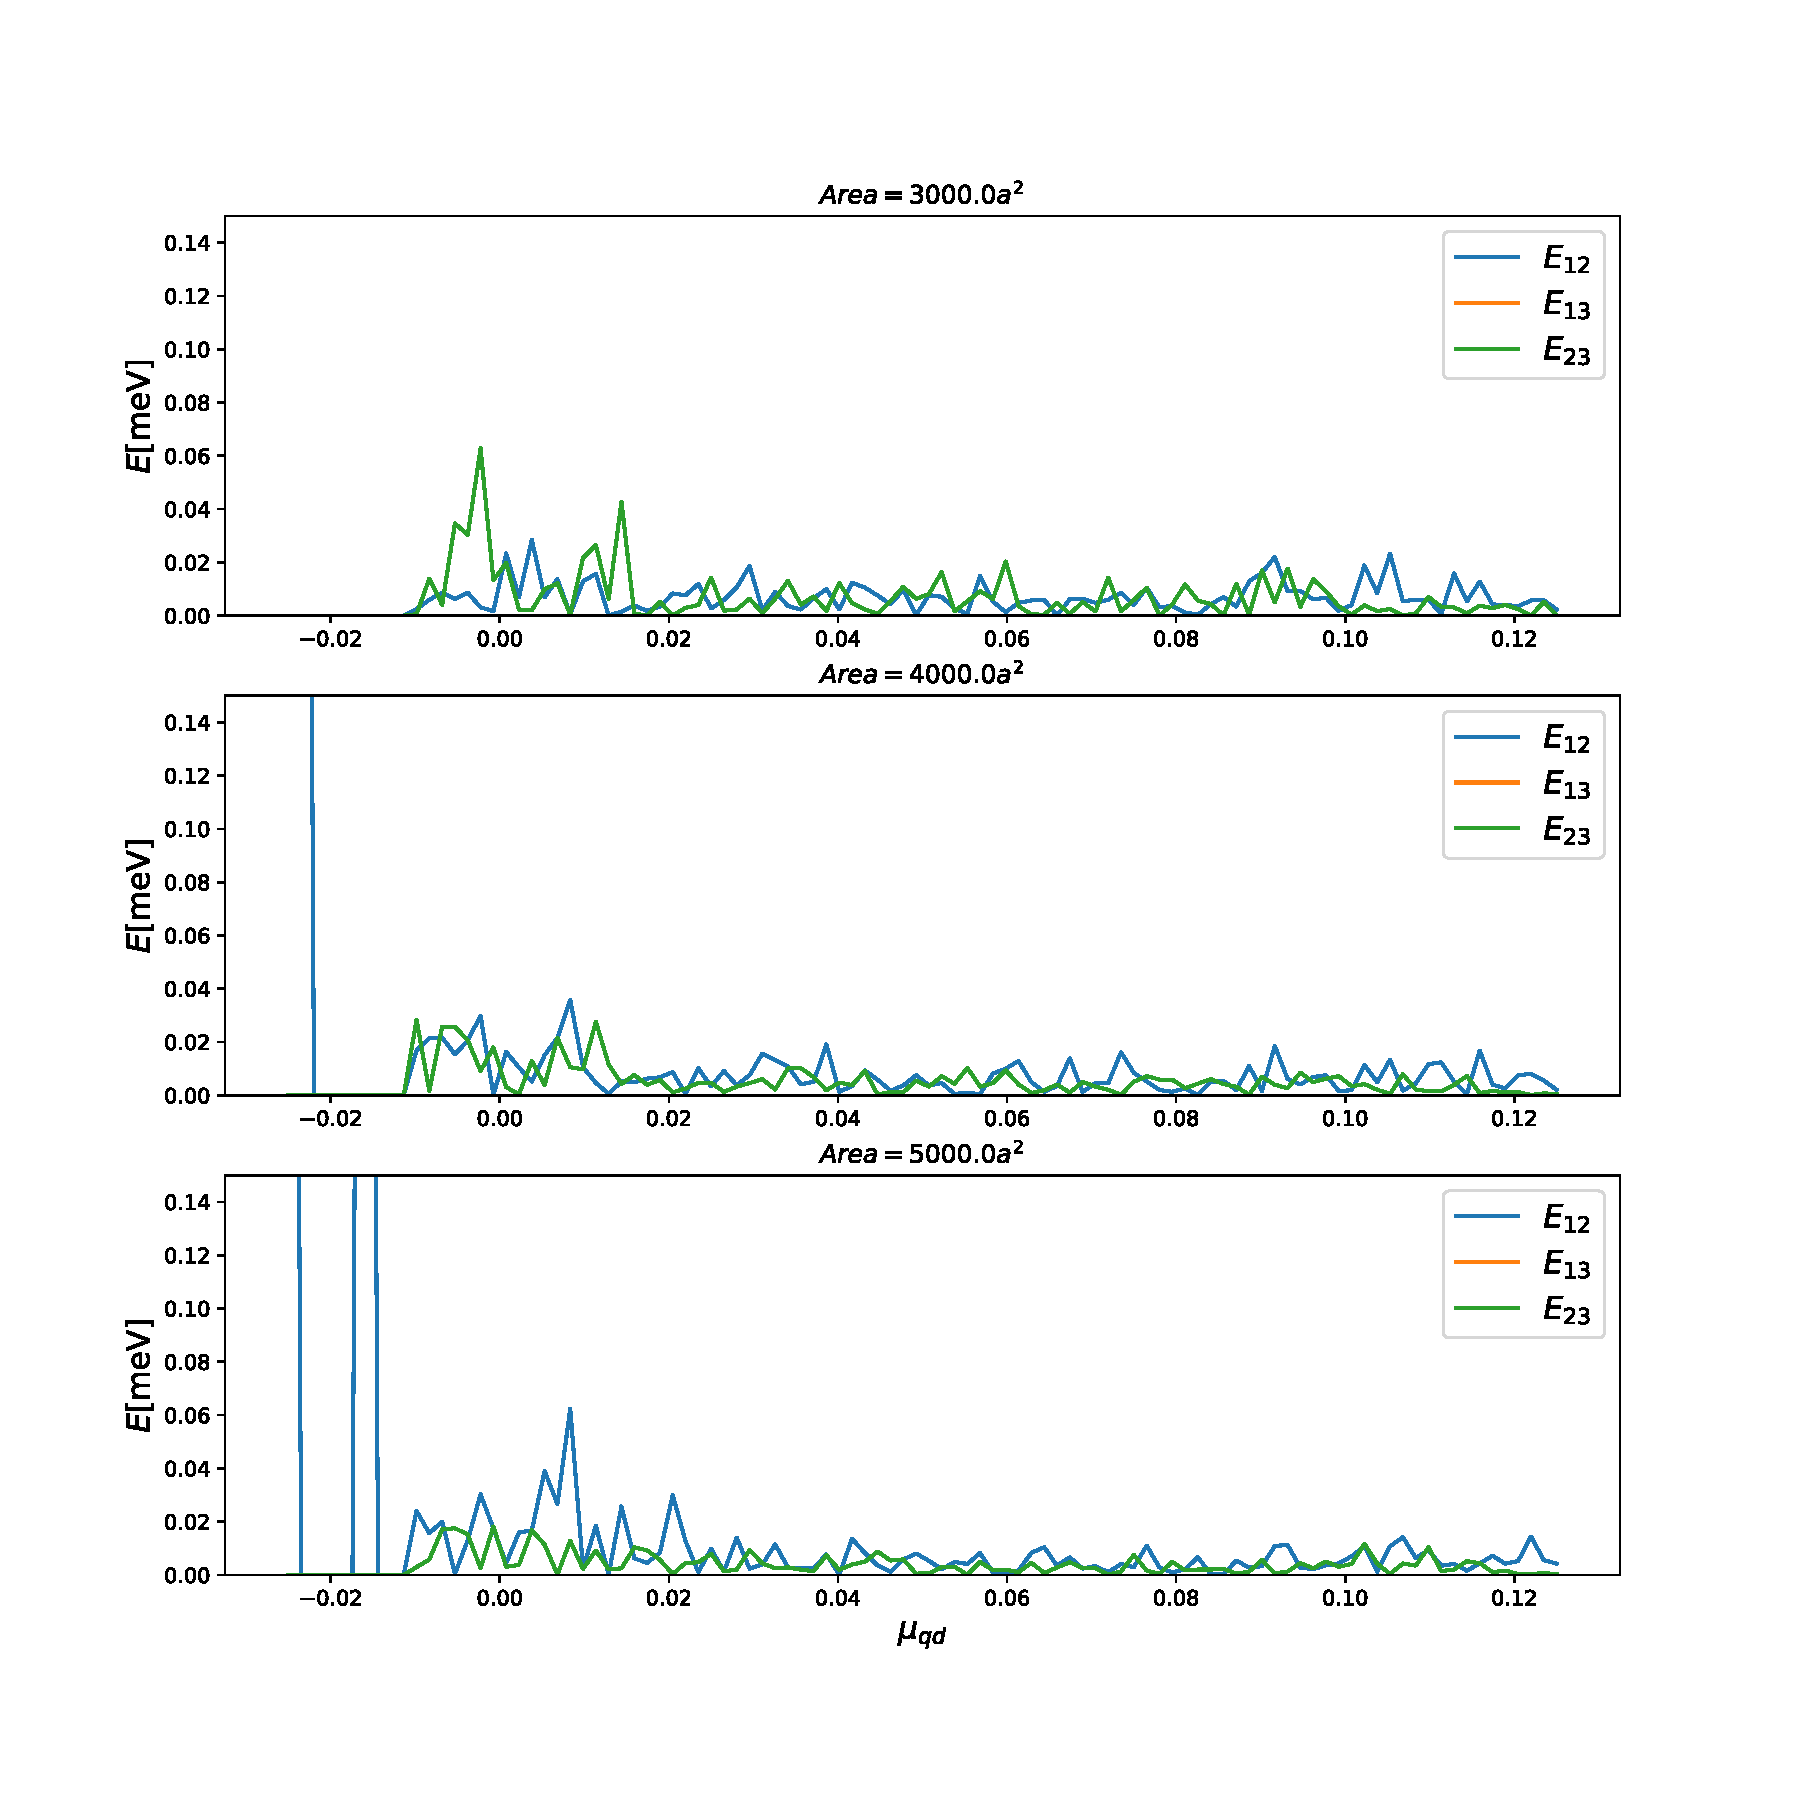
\includegraphics[width=\linewidth]{figures/half_ring_coupling.pdf}
  \caption{Coupling of all pairs of MBS as a function of the cavity chemical potential, $\mu_{qd}$, for a half ring geometry. The area of the scattering region is increased for each plot. The green and orange curves are completely overlaping since the system is symmetric.}
  \label{fig:half_ring}
\end{figure}

\subsection{Broad parametric geometries}

In contrast to the narrow case, a broader scattering region allows for longer trajectories that couple different pairs of MBS. Furthermore, a parametric shape allows us to control the trajectories in such a way that the coupling of a given pair is enhanced. That is the case of a triangular cavity where the angle of the diagonal sides, $\theta$, is varied. The coupling of all MBS pairs as a function of the cavity chemical potential is shown in Fig. \ref{fig:angles} for the lowest lead band. One can observe that there's a clear angle dependence, and that the coupling is much larger than in the narrow case. For small angles around $\theta=0.15\pi$, one can observe that the coupling between all pairs of MBS is comparable. In particular, there are cavity levels that couple equality to all MBS pairs. As the angle is increased, one pair dominates over the others. The largest coupling values are reached for $E_{12}$, i.e. left and right MBS, around $\theta=0.35\pi$.  As the angle is further increased, $E_{13}$ and $E_{23}$ dominates over $E_{12}$.

\begin{figure}[h!]
  \centering
  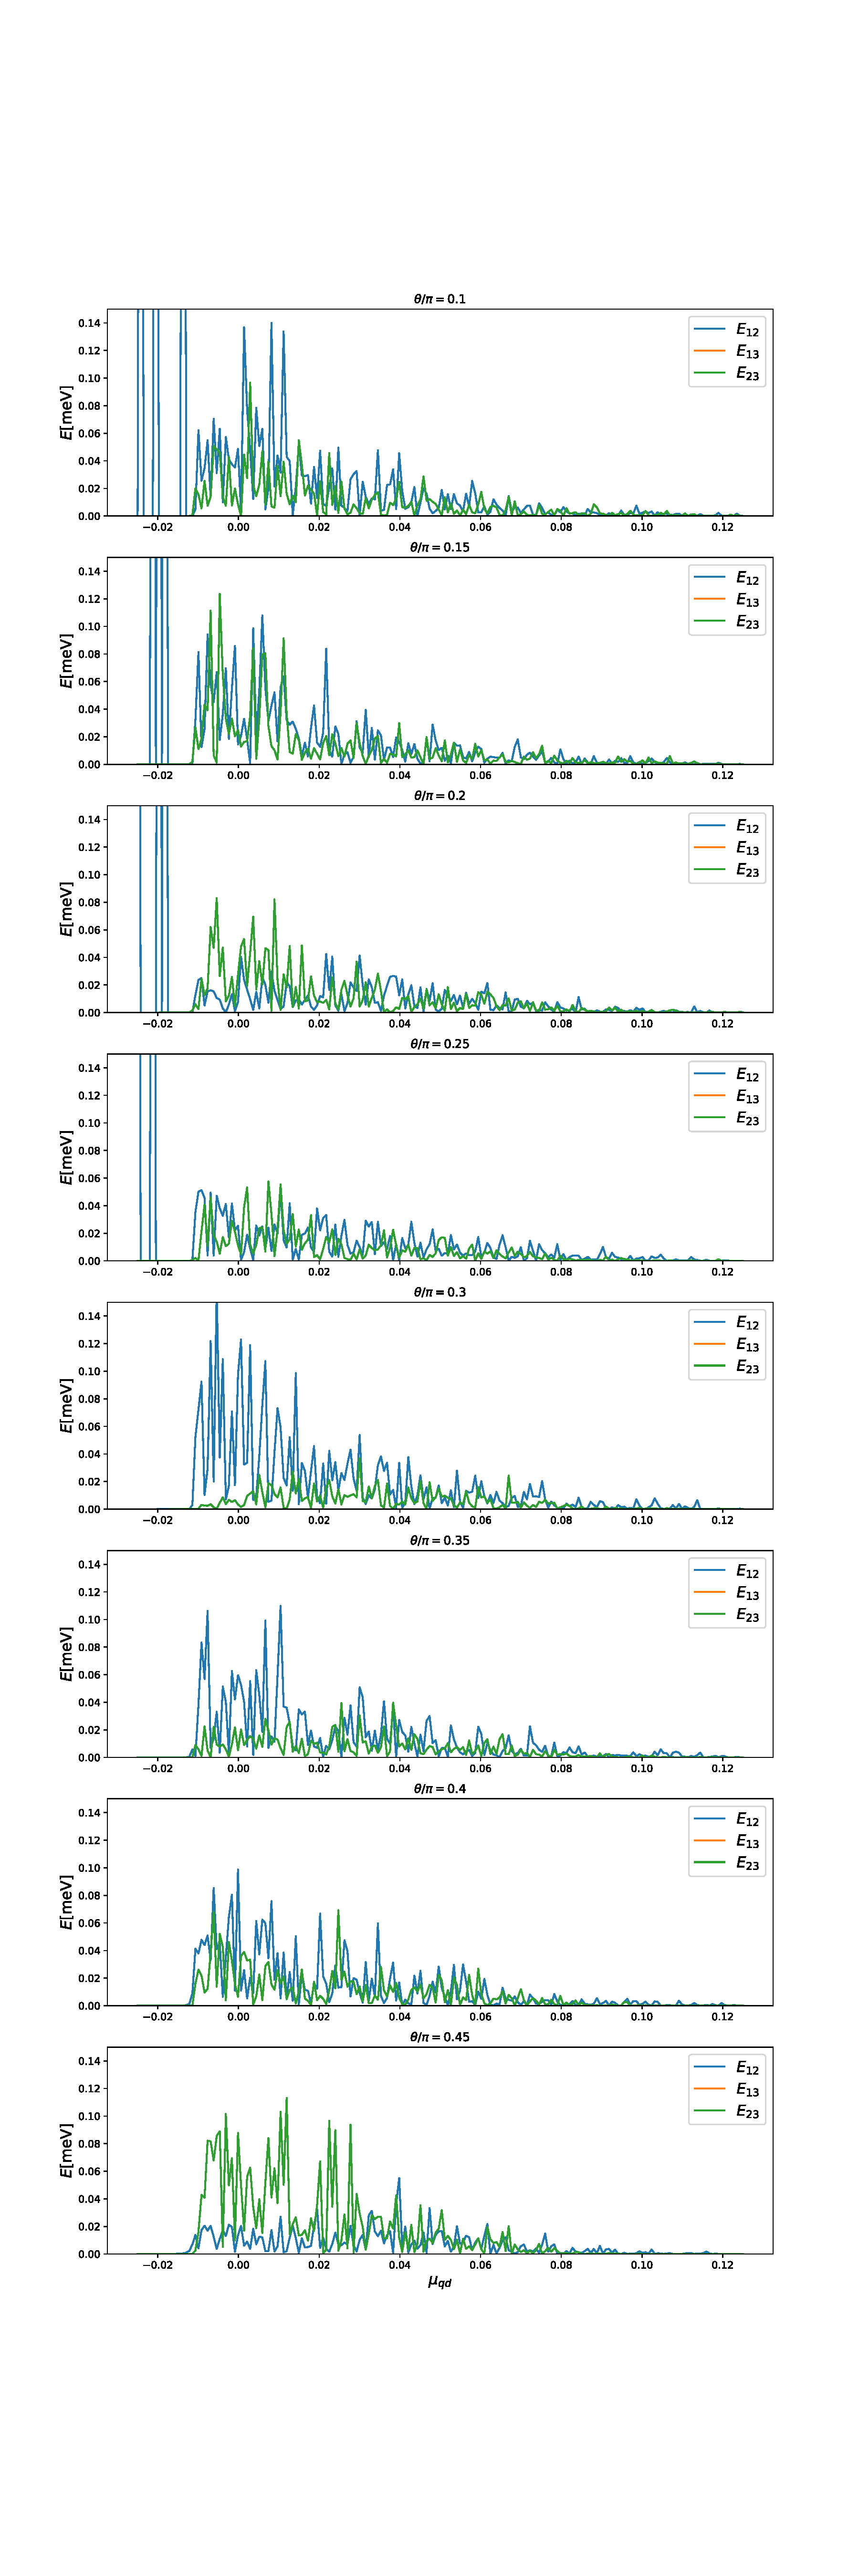
\includegraphics[width=\linewidth]{figures/triangle_coupling_lowest_band.pdf}
  \caption{Coupling of all pairs of MBS as a function of the cavity chemical potential for the lowest nanowire sub band. The angle is varied for each plot.}
  \label{fig:angles}
\end{figure}

\section{To do?}

\begin{itemize}
\item Add a half-billard shape.
\item Complete calculations for all shapes using the bound state algorithm. It is not working yet.
\item Find a way to characterise the cavity states that couple the most to MBS. Mert suggested using local FT to find trajectories, or the $IPR=\sum_{i} |\psi_{i}|^{4}$ to study how localised they are. 
\item Also, there are two kinds of states in a ballistic cavity: whispering modes that go along the borders of the shape, and bouncing ball states that move back and forth between the boundaries. Position of the leads determines which states couple.
\item Make gate configuration for other shapes besides the triangular.
\item Add disorder to the system. Charge noise? chemical potential noise? irregular border in etched structures? how to add electrostatics to that?
\end{itemize}

\bibliography{bibliography}

\end{document}
